\chapter{Bayes minimum risk}\label{ch:6}

\begin{remark}{Outline}
In this chapter, we propose the Bayes minimum risk algorithm. The method 
consists in quantifying tradeoffs between various decisions using probabilities and the costs that 
accompany such decisions. First, in Section~\ref{sec:6:bmr}, we present the Bayes minimum risk 
algorithm. Then, in Section~\ref{sec:6:prob}, we discuss the impact of calibrating the probabilities 
in the model. Finally, in Section~\ref{sec:6:experiments},  using the five real-world cost-sensitive 
databases, we compare the results of the proposed algorithm, against state-of-the-art methods.
\end{remark}


\section{Bayes minimum risk model}
\label{sec:6:bmr}

% % As decribed in Section \ref{sec:3:cs}, state-of-the-art example dependent techniques, only 
% introduce the cost by modifying the training set. In \citep{CorreaBahnsen2013,CorreaBahnsen2014}, 
% we proposed a cost-sensitive model called Bayes minimum risk classifier ($BMR$).  

As defined in \citep{Ghosh2006}, the BMR classifier is a decision model based on quantifying 
tradeoffs between various decisions using probabilities and the costs that accompany such decisions. 
This is done in a way that for each example the expected losses are minimized. In  what follows, we 
consider the probability estimates $\hat p_i$ as known, regardless of the algorithm used to 
calculate them.  The risk that accompanies each decision is calculated using the cost matrix 
as described in \tablename{ \ref{tab:3:cost_matrix}}. In the specific framework of binary 
classification, the risk of predicting the example $i$ as negative is 
\begin{equation}
  R(c_i=0|\mathbf{x}_i)=C_{TN_i}(1-\hat p_i)+C_{FN_i} \cdot \hat p_i, 
\end{equation}
and
\begin{equation}
  R(c_i=1|\mathbf{x}_i)=C_{TP_i} \cdot \hat p_i + C_{FP_i}(1- \hat p_i), 
\end{equation}
is the risk when predicting the example as positive, where $\hat p_i$ is the estimated positive 
probability for example $i$. Subsequently, if 
\begin{equation}
  R(c_i=0|\mathbf{x}_i) \le R(c_i=1|\mathbf{x}_i), 
\end{equation}
then  the example $i$ is classified as negative. This means that the risk associated with the 
decision $c_i$ is lower than the risk associated with classifying it as positive. 


\section{Calibration of probabilities}
\label{sec:6:prob}

When using the output of a binary classifier as a basis for decision making, there is a 
need for a probability that not only separates well between positive and negative examples, but 
that also assesses the real probability of the event \citep{cohen2004}.

In this section, two methods for calibrating probabilities are explained. First, the method proposed 
in \citep{Elkan2001} to adjust the probabilities based on the   difference in bad rates  between the 
training and testing datasets.  Then, the method proposed in \cite{Hernandez-Orallo2012}, in which 
calibrated probabilities are extracted after modifying the ROC curve using the ROC convex hull 
methodology, is described.
 
\subsection{Calibration due to a change in base rates}

One of the reasons why a probability may not be calibrated is because the algorithm is trained 
using a dataset with a different base (or positive) rate than the one on the evaluation dataset.  
This is something common in machine learning since using under-sampling or over-sampling is a 
typical method to solve problems such as class imbalance and cost sensitivity \citep{Hulse2007}.
  
In order to solve this and find probabilities that are calibrated, in \citep{Elkan2001} a formula  
that corrects the probabilities based on the difference of the base rates is proposed.  The 
objective is using $\hat p$ which was estimated using a population with base rate $\pi_1$,
to find $\hat p'$ for the real population which has a base rate $\pi_1'$. A solution for $\hat p'$ 
is given as follows:
\begin{equation}
  \hat p'=\pi_1' \frac{\hat p - \hat p \pi_1}{\pi_1- \pi_1 \hat p +\pi_1' \hat p - \pi_1 \pi_1'}.
\end{equation}

% Nevertheless, a strong assumption is made by taking: $P'(x|j=1)=P(x|j=1)$} and 
% \mbox{$P'(x|j=0)=P(x|j=0)$}, meaning that there
%   is no change in the example probability within the positive and negative
%   subpopulations density functions.
  
\subsection{Calibration using the ROC convex hull}

In order to illustrate the ROC convex hull approach proposed in \citep{Hernandez-Orallo2012},
let us consider the set of probabilities given in \figurename{~\ref{tab:6:example_prob}}.
Their corresponding  ROC curve  is shown in \figurename{~\ref{fig:6:ROC_1}}.  It can be seen that 
this set of probabilities is not calibrated, since when $fpr=0.1$ there is a positive example  
followed by 2 negative examples. This inconsistency is represented in the ROC curve as a non convex 
segment  over the curve.
  
\begin{figure}[!t]
\hskip 0.5cm
\hbox{
  \vtop{
    \hbox{
      \subfloat[Set of probabilities and their respective class label]{
   \footnotesize
	\begin{tabular}{cc}
	\hline
	Probability & Label\\
	\hline
	0.0&	0\\
	0.1&	1\\
	0.2&	0\\
	0.3&	0\\
	0.4&	1\\
	0.5&	0\\
	0.6&	1\\
	0.7&	1\\
	0.8&	0\\
	0.9&	1\\
	1.0&	1\\
	\hline
	\end{tabular}\label{tab:6:example_prob}
      }
    }
  }\hskip 0.5cm
  \vtop{\vskip -2.5cm
    \subfloat[ROC curve of the set of probabilities]{
      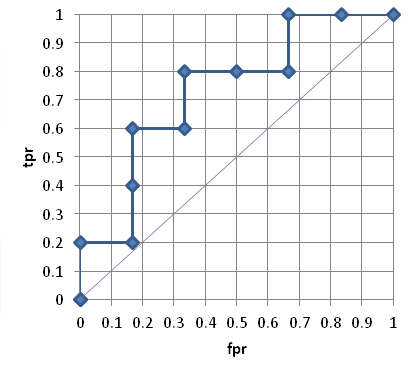
\includegraphics[scale=0.5]{ch6_fig2}\label{fig:6:ROC_1}
    }%
  }%
}
\vskip 1.5cm

\hbox{ 
  \vtop{ \vskip 0.5cm
    \hbox{
      \subfloat[Convex hull of the ROC curve]{
	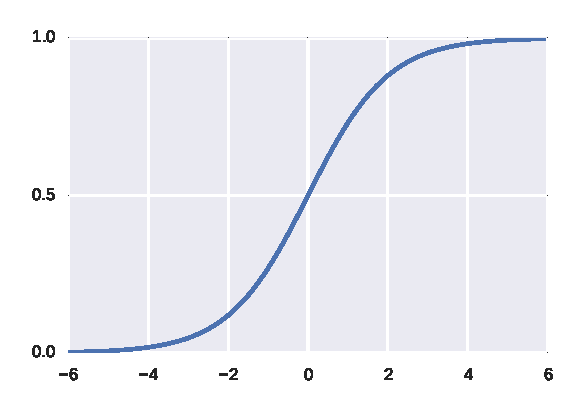
\includegraphics[scale=0.5]{ch6_fig1}\label{fig:6:ROC_2}
      }
    }
  }\hskip 1cm
  \vtop{ \vskip -1cm
    \subfloat[Calibrated probabilities]{
   \footnotesize
	\begin{tabular}{cc}
	\hline
	Prob & Cal Prob\\
	\hline
	0.0&	0\\
	0.1&	0.333\\
	0.2&	0.333\\
	0.3&	0.333\\
	0.4&	0.5\\
	0.5&	0.5\\
	0.6&	0.666\\
	0.7&	0.666\\
	0.8&	0.666\\
	0.9&	1\\
	1.0&	1\\
	\hline
	\end{tabular}\label{fig:6:cal_prob} 
    }
  }
}
\caption{Estimation of calibrated probabilities using the ROC convex hull.}\label{fig:6:rocch}
\end{figure}

In order to obtain a set of calibrated probabilities, first the ROC curve must be modified in 
order to be convex. The way to do that, is to find the convex \mbox{hull 
\citep{Hernandez-Orallo2012}} to find the minimal convex set containing the different 
points of the ROC curve. In \figurename{~\ref{fig:6:ROC_2}}, the convex hull algorithm is applied 
to the previously evaluated ROC curve shown in \figurename{~\ref{fig:6:ROC_1}}. It is shown that 
the new curve is convex, and includes all the points of the previous ROC curve.

Now that there is a new convex ROC curve or ROCCH, the calibrated probabilities can be extracted 
as shown in  \figurename{~\ref{fig:6:cal_prob}}. The procedure to extract the new probabilities is 
to first group the probabilities according to the points in the ROCCH curve, and then make the 
calibrated  probabilities be the slope of the ROCCH for each group.
  
   
\section{Experiments}
\label{sec:6:experiments}

For the experiments we use five datasets from four different real world example-dependent 
cost-sensitive problems: Credit card fraud detection (see Section~\ref{sec:4:fraud}), credit 
scoring (see Section~\ref{sec:4:creditscoring}), churn modeling (see Section~\ref{sec:5:churn}) and 
direct marketing (see Section~\ref{sec:5:directmarketing}). The different datasets are summarized 
in \tablename{~\ref{tab:4:databases}} and \tablename{~\ref{tab:5:databases}}.

For the experiments, we first used three classification algorithms, decision tree ($DT$), logistic 
  regression ($LR$) and random forest ($RF$). Using the implementation of \textit{Scikit-learn} 
  \citep{Pedregosa2011}, each algorithm is trained using the different training sets: training 
  ($t$), under-sampling ($u$), cost-proportionate rejection-sampling  ($r$) \citep{Zadrozny2003}   
  and   cost-proportionate over-sampling ($o$) \citep{Elkan2001}. Afterwards,  we evaluate the 
  results of  the algorithms using $BMR$ methods. In particular, we   check the impact on the 
  results of the different calibration methods. The implementation of the cost-sensitive algorithms 
  is done using the \textit{CostCla} library, see Appendix~\ref{ch:A}.
  
  \begin{table}[!b]
    \centering
    \footnotesize
    \begin{tabular}{l l r@{\hskip 0in}c@{\hskip 0in}l r@{\hskip 0in}c@{\hskip 0in}l r@{\hskip 
    0in}c@{\hskip 0in}l  } %sum 7.7
    \hline
    \bf{Family} & \bf{Algorithm} & \multicolumn{3}{c}{\bf{Fraud}} & 
    \multicolumn{3}{c}{\bf{Churn}} & \multicolumn{3}{c}{\bf{Credit 1}} \\ 
    \hline
CI&DT-t & 0.3176 &$\pm$& 0.0357 & -0.0018 &$\pm$& 0.0194 & 0.1931 &$\pm$& 0.0087\\ 
&LR-t & 0.0092 &$\pm$& 0.0002 & -0.0001 &$\pm$& 0.0002 & 0.0177 &$\pm$& 0.0126\\ 
&RF-t & 0.3342 &$\pm$& 0.0156 & -0.0026 &$\pm$& 0.0079 & 0.1471 &$\pm$& 0.0071\\ 
&DT-u & 0.5239 &$\pm$& 0.0118 & -0.0389 &$\pm$& 0.0583 & 0.3287 &$\pm$& 0.0125\\ 
&LR-u & 0.1243 &$\pm$& 0.0387 & 0.0039 &$\pm$& 0.0492 & 0.4118 &$\pm$& 0.0313\\ 
&RF-u & 0.5684 &$\pm$& 0.0097 & 0.0433 &$\pm$& 0.0533 & 0.4981 &$\pm$& 0.0079\\ 
\hline 
CPS&DT-r & 0.3439 &$\pm$& 0.0453 & 0.0054 &$\pm$& 0.0568 & 0.3310 &$\pm$& 0.0126\\ 
&LR-r & 0.3077 &$\pm$& 0.0301 & 0.0484 &$\pm$& 0.0375 & 0.3965 &$\pm$& 0.0263\\ 
&RF-r & 0.3812 &$\pm$& 0.0264 & 0.1056 &$\pm$& 0.0412 & \bf{0.4989} &\bf{$\pm$}& \bf{0.0080}\\ 
&DT-o & 0.3172 &$\pm$& 0.0274 & 0.0251 &$\pm$& 0.0195 & 0.1738 &$\pm$& 0.0092\\ 
&LR-o & 0.2793 &$\pm$& 0.0185 & 0.0316 &$\pm$& 0.0228 & 0.3301 &$\pm$& 0.0109\\ 
&RF-o & 0.3612 &$\pm$& 0.0295 & 0.0205 &$\pm$& 0.0156 & 0.2128 &$\pm$& 0.0081\\ 
\hline 
BMR&DT-t-BMR & 0.6045 &$\pm$& 0.0386 & 0.0226 &$\pm$& 0.0200 & 0.1931 &$\pm$& 0.0087\\ 
&LR-t-BMR & 0.4552 &$\pm$& 0.0203 & 0.0872 &$\pm$& 0.0308 & 0.1973 &$\pm$& 0.0404\\ 
&RF-t-BMR & 0.6175 &$\pm$& 0.0149 & 0.0435 &$\pm$& 0.0356 & 0.4878 &$\pm$& 0.0082\\ 
\hline 
CAL&DT-t-BMR-cal & 0.5936 &$\pm$& 0.0386 & 0.0298 &$\pm$& 0.0145 & 0.1054 &$\pm$& 0.0358\\ 
BMR&LR-t-BMR-cal & 0.0897 &$\pm$& 0.0203 & \bf{0.1082} &\bf{$\pm$}& \bf{0.0316} & 0.2189 &$\pm$& 
0.0541\\ 
&RF-t-BMR-cal & \bf{0.6414} &\bf{$\pm$}& \bf{0.0154} & 0.0856 &$\pm$& 0.0354 & 0.4924 &$\pm$& 
0.0087\\  
\hline
  \multicolumn{11}{c}{(Models with the highest savings are marked in bold)}
  \end{tabular}
    \caption{Results of the algorithms measured by savings}
    \label{tab:6:results_savings}
  \end{table}
  
The results are shown in \tablename{ \ref{tab:6:results_savings}}. First, when observing  the 
results of the cost-insensitive methods ($CI$), that is, $DT$, $LR$ and $RF$ algorithms trained 
on the $t$ and $u$ sets, the $RF$ algorithm produces the best result by savings in three out of 
the five sets, followed by the $LR-u$. It is also clear that the results on the $t$ dataset are 
not as good as the ones on the $u$ dataset, this is highly related to the unbalanced distribution 
of the positives and negatives in all the databases.  
  
\begin{table}[!t]
    \centering
    \footnotesize
    \begin{tabular}{l l r@{\hskip 0in}c@{\hskip 0in}l r@{\hskip 0in}c@{\hskip 0in}l  } %sum 7.7
    \hline
    \bf{Family} & \bf{Algorithm} &  \multicolumn{3}{c}{\bf{Credit 2}} 
& \multicolumn{3}{c}{\bf{Marketing}} \\ 
    \hline
CI&DT-t & -0.0616 &$\pm$& 0.0229 & -0.2342 &$\pm$& 0.0609\\ 
&LR-t & 0.0039 &$\pm$& 0.0012 & -0.2931 &$\pm$& 0.0602\\ 
&RF-t & 0.0303 &$\pm$& 0.0040 & -0.2569 &$\pm$& 0.0637\\ 
&DT-u & -0.1893 &$\pm$& 0.0314 & -0.0278 &$\pm$& 0.0475\\ 
&LR-u & 0.1850 &$\pm$& 0.0231 & 0.2200 &$\pm$& 0.0376\\ 
&RF-u & 0.1237 &$\pm$& 0.0228 & 0.1227 &$\pm$& 0.0443\\ 
\hline 
CPS&DT-r & 0.0724 &$\pm$& 0.0212 & 0.1960 &$\pm$& 0.0527\\ 
&LR-r & 0.2650 &$\pm$& 0.0115 & 0.4210 &$\pm$& 0.0267\\ 
&RF-r & 0.3055 &$\pm$& 0.0106 & 0.3840 &$\pm$& 0.0360\\ 
&DT-o & 0.0918 &$\pm$& 0.0225 & -0.2598 &$\pm$& 0.0559\\ 
&LR-o & 0.2554 &$\pm$& 0.0090 & 0.3129 &$\pm$& 0.0277\\ 
&RF-o & 0.2242 &$\pm$& 0.0070 & -0.1782 &$\pm$& 0.0618\\ 
\hline 
BMR&DT-t-BMR & -0.0616 &$\pm$& 0.0230 & -0.2185 &$\pm$& 0.0611\\ 
&LR-t-BMR & 0.3119 &$\pm$& 0.0089 & 0.4915 &$\pm$& 0.0090\\ 
&RF-t-BMR & 0.3027 &$\pm$& 0.0096 & 0.3722 &$\pm$& 0.0263\\ 
\hline 
CAL&DT-t-BMR-cal & 0.2740 &$\pm$& 0.0067 & 0.4598 &$\pm$& 0.0089\\ 
BMR&LR-t-BMR-cal & \bf{0.3148} &\bf{$\pm$}& \bf{0.0094} & \bf{0.4973} &\bf{$\pm$}& \bf{0.0084}\\ 
&RF-t-BMR-cal & 0.3133 &$\pm$& 0.0094 & 0.4807 &$\pm$& 0.0093\\ 

\hline 
  \multicolumn{8}{c}{(Models with the highest savings are marked in bold)}
  \end{tabular}
    \caption{Continuation of \tablename{~\ref{tab:6:results_savings}}.}
    \label{tab:6:results_savings2}
  \end{table}
  
In the case of cost-proportionate sampling methods ($CPS$), specifically the 
cost-proportionate rejection sampling ($r$) and cost-proportionate over 
sampling ($o$), it is observed that in four cases the savings increase quite 
significantly. It is on the fraud detection database where these methods do not outperform the 
algorithms trained on the under-sampled set. This may be related to the fact that in this 
database the initial percentage of positives is 1.5\% which is similar to the percentage in the 
$r$ and   $o$ sets. However, it is 50.42\% in the $u$ set, which may help explain why this method 
performs much better as measured by savings.

\begin{figure}[!t]
  \centering
  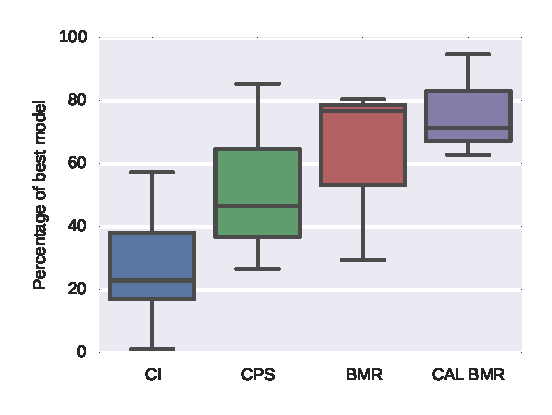
\includegraphics{ch6_fig3}
  \caption{\textbf{Comparison of the average savings of the algorithms versus the 
    highest savings by family of classifiers.} When the probabilities are calibrated there is a 
    significant increase in savings.}
  \label{fig:6:comparison_family}
\end{figure}

  \begin{table}[!t]
    \centering
    \footnotesize
    \begin{tabular}{l l r@{\hskip 0in}c@{\hskip 0in}l r@{\hskip 0in}c@{\hskip 0in}l r@{\hskip 
    0in}c@{\hskip 0in}l  } %sum 7.7
    \hline
    \bf{Family} & \bf{Algorithm} & \multicolumn{3}{c}{\bf{Fraud}} & 
    \multicolumn{3}{c}{\bf{Churn}} & \multicolumn{3}{c}{\bf{Credit 1}} \\ 
    \hline
CI&DT-t & 0.0134 &$\pm$& 0.0005 & 0.0932 &$\pm$& 0.0054 & 0.1054 &$\pm$& 0.0016\\ 
&LR-t & 0.0440 &$\pm$& 0.0008 & 0.0449 &$\pm$& 0.0025 & 0.0598 &$\pm$& 0.0016\\ 
&RF-t & 0.0064 &$\pm$& 0.0002 & 0.0532 &$\pm$& 0.0027 & 0.0519 &$\pm$& 0.0007\\ 
&DT-u & 0.1424 &$\pm$& 0.0071 & 0.4152 &$\pm$& 0.0205 & 0.3141 &$\pm$& 0.0052\\ 
&LR-u & 0.1872 &$\pm$& 0.0195 & 0.2439 &$\pm$& 0.0139 & 0.1718 &$\pm$& 0.0088\\ 
&RF-u & 0.0724 &$\pm$& 0.0007 & 0.2442 &$\pm$& 0.0134 & 0.1565 &$\pm$& 0.0019\\ 
\hline 
CPS&DT-r & 0.2041 &$\pm$& 0.0111 & 0.3595 &$\pm$& 0.0185 & 0.2884 &$\pm$& 0.0054\\ 
&LR-r & 0.1726 &$\pm$& 0.0098 & 0.1906 &$\pm$& 0.0112 & 0.1448 &$\pm$& 0.0063\\ 
&RF-r & 0.1764 &$\pm$& 0.0127 & 0.1964 &$\pm$& 0.0101 & 0.1374 &$\pm$& 0.0028\\ 
&DT-o & 0.1264 &$\pm$& 0.0102 & 0.0963 &$\pm$& 0.0048 & 0.1020 &$\pm$& 0.0014\\ 
&LR-o & 0.2158 &$\pm$& 0.0098 & 0.1136 &$\pm$& 0.0025 & 0.1134 &$\pm$& 0.0014\\ 
&RF-o & 0.1694 &$\pm$& 0.0146 & 0.0701 &$\pm$& 0.0031 & 0.0550 &$\pm$& 0.0008\\ 
\hline 
BMR&DT-t-BMR & 0.0134 &$\pm$& 0.0005 & 0.0932 &$\pm$& 0.0054 & 0.1054 &$\pm$& 0.0016\\ 
&LR-t-BMR & 0.0440 &$\pm$& 0.0008 & 0.0449 &$\pm$& 0.0025 & 0.0598 &$\pm$& 0.0016\\ 
&RF-t-BMR & 0.0064 &$\pm$& 0.0002 & 0.0532 &$\pm$& 0.0027 & 0.0519 &$\pm$& 0.0007\\ 
\hline 
CAL&DT-t-BMR-cal & 0.0098 &$\pm$& 0.0004 & 0.0448 &$\pm$& 0.0029 & 0.0604 &$\pm$& 0.0009\\ 
BMR&LR-t-BMR-cal & 0.0148 &$\pm$& 0.0007 & \bf{0.0444} &\bf{$\pm$}& \bf{0.0025} & 0.0590 &$\pm$& 
0.0018\\ 
&RF-t-BMR-cal & \bf{0.0058} &\bf{$\pm$}& \bf{0.0003} & 0.0446 &$\pm$& 0.0026 & \bf{0.0514} 
&\bf{$\pm$}& \bf{0.0008}\\ 
\hline
  \multicolumn{11}{c}{(Models with the lowest Brier score are marked as bold)}
  \end{tabular}
    \caption{Results of the algorithms measured by Brier score}
    \label{tab:6:results_brier}
\end{table}

Afterwards, in the case of the $BMR$ algorithms, the results show that this method outperforms 
the previous ones in four cases and has almost the same result in the other set. In the fraud 
detection  set, the results are better, since the savings of the three classification 
algorithms increase when using this methodology. Moreover, we found that by calibrating the 
probabilities, the results of the Bayes minimum risk increase. In 
\figurename{~\ref{fig:6:comparison_family}}, we compare the different families of algorithms, by 
calculating in each dataset the performance of the methods compared with the best method. First, it 
is shown the huge difference of using only cost-insensitive methods, compared with any of the 
cost-sensitive families. Furthermore, the Bayes minimum risk methods outperforms the 
cost-proportionate sampling methods.

\begin{table}[t]
    \centering
    \footnotesize
    \begin{tabular}{l l r@{\hskip 0in}c@{\hskip 0in}l r@{\hskip 0in}c@{\hskip 0in}l  } %sum 7.7
    \hline
    \bf{Family} & \bf{Algorithm} &  \multicolumn{3}{c}{\bf{Credit 2}} 
& \multicolumn{3}{c}{\bf{Marketing}} \\ 
    \hline
CI&DT-t & 0.3103 &$\pm$& 0.0041 & 0.1924 &$\pm$& 0.0035\\ 
&LR-t & 0.1511 &$\pm$& 0.0016 & 0.0960 &$\pm$& 0.0018\\ 
&RF-t & 0.1525 &$\pm$& 0.0016 & 0.1090 &$\pm$& 0.0018\\ 
&DT-u & 0.4526 &$\pm$& 0.0057 & 0.4125 &$\pm$& 0.0062\\ 
&LR-u & 0.2317 &$\pm$& 0.0017 & 0.2016 &$\pm$& 0.0027\\ 
&RF-u & 0.2325 &$\pm$& 0.0024 & 0.2256 &$\pm$& 0.0036\\ 
\hline 
CPS&DT-r & 0.5516 &$\pm$& 0.0070 & 0.3581 &$\pm$& 0.0111\\ 
&LR-r & 0.2657 &$\pm$& 0.0051 & 0.2029 &$\pm$& 0.0055\\ 
&RF-r & 0.3613 &$\pm$& 0.0055 & 0.2123 &$\pm$& 0.0054\\ 
&DT-o & 0.4550 &$\pm$& 0.0039 & 0.1904 &$\pm$& 0.0028\\ 
&LR-o & 0.2258 &$\pm$& 0.0023 & 0.1517 &$\pm$& 0.0013\\ 
&RF-o & 0.3283 &$\pm$& 0.0030 & 0.1190 &$\pm$& 0.0016\\ 
\hline 
BMR&DT-t-BMR & 0.3103 &$\pm$& 0.0041 & 0.1924 &$\pm$& 0.0035\\ 
&LR-t-BMR & 0.1511 &$\pm$& 0.0016 & 0.0960 &$\pm$& 0.0018\\ 
&RF-t-BMR & 0.1525 &$\pm$& 0.0016 & 0.1090 &$\pm$& 0.0018\\ 
\hline 
CAL&DT-t-BMR-cal & 0.1586 &$\pm$& 0.0019 & 0.1075 &$\pm$& 0.0017\\ 
BMR&LR-t-BMR-cal & \bf{0.1505} &\bf{$\pm$}& \bf{0.0016} & \bf{0.0952} &\bf{$\pm$}& \bf{0.0017}\\ 
&RF-t-BMR-cal & 0.1510 &$\pm$& 0.0016 & 0.0999 &$\pm$& 0.0019\\ 
\hline 
  \multicolumn{8}{c}{(Models with the lowest Brier score are marked as bold)}
  \end{tabular}
    \caption{Continuation of \tablename{~\ref{tab:6:results_brier}}.}
    \label{tab:6:results_savings2}
  \end{table}

  
Moreover, we evaluate the Brier score of the different algorithms. The objective of this, is 
because as mention in  \citep{cohen2004}, when using the output of a binary classifier as a basis 
for decision making, there is a need for a probability that not only separates well between 
positive 
and negative examples, but that also assesses the real probability of the event. The results are 
shown in \tablename{~\ref{tab:6:results_brier}}. First of all, as expected, the logistic regression 
models are very well calibrated regardless of the dataset used for train them. This is because, the 
logistic regression algorithm is intended to estimate the most reliable probabilities as we will 
discuss in \chaptername{~\ref{ch:7}}.

When comparing the results of the Bayes minimum risk with and without calibration, it is clear that 
the calibration of the probabilities lead to a lower Brier score as shown in 
\figurename{~\ref{fig:6:comparison_family_brier}}. Interestingly, the results of Brier score 
and the savings are highly correlated, confirming the intuition behind the need to calibrate the 
probabilities before using the Bayes minimum risk method.

\begin{figure}[!t]
  \centering
  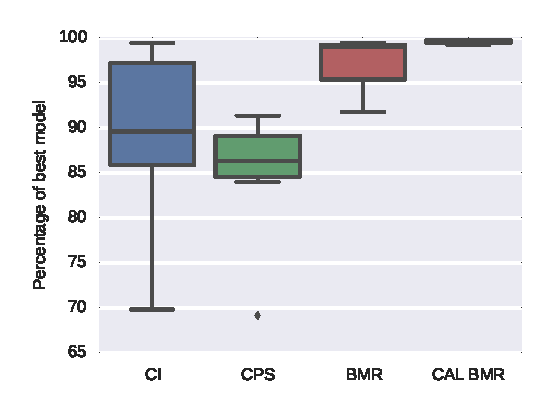
\includegraphics{ch6_fig4}
  \caption{\textbf{Comparison of the average Brier score of the algorithms versus the 
    lowest Brier score by family of classifiers.} Overall, the models that are calibrated are 
indeed the ones with the best Brier score.}
  \label{fig:6:comparison_family_brier}
\end{figure}


  
  
  